一个 MR job 通常会把输入数据划分成独立的 chunks. 每个 chunk 会被 map tasks 并行地处理. 然后 MR 这个框架会对 map 的输出进行排序, 然后输入给 reduce tasks. 通常输入和输出都存储在文件系统中. tasks 的调度由 MR 框架负责, 监控它们的执行并再执行失败的任务. MR 框架中有一个 ResourceManager, 每个 worker 节点一个 NodeManager, 每个应用一个 MRAppMaster. 最低程度上,一个 MR 应用等于: 输入/输出 + map 和 reduce 函数(实现了相应的接口)+ 关于 job 的一些参数 (job configuration). 有了 job 后, Hadoop 的 job-client 会提交 job (即可执行文件) 以及配置给 ResourceManager, 它会把这些\textbf{可执行文件}和\textbf{配置}分发到各个 workers, 调度和监控 tasks 的执行并把状态数据发送给 job-client.

\subsection{一些基本概念}

\par{\textbf{\textcolor{red}{Mapper}}}$\quad$ 对于 InputFormat 生成的每个 InputSplit, MR 都会产生一个对应的 map task 进行处理. map 输入输出的类型和数量不一定要相同. 对于 mapper 输出的 k-v pairs. 并不是直接输入给 reducer, 而是会由框架进行一次处理后在输入给 reducer. 处理的方式: 按照 key 对输出进行聚合. Mapper 任务的输出还会再进行一次排序然后进行划分, 每个 reducer 一个 partition. 如果没有 Reducer, 则 mapper 的输出会直接写道文件系统中, 此时则不会对输出进行排序. 

\par{\textbf{\textcolor{red}{Reducer}}}$\quad$ Reducer 主要分成三成三个阶段: shuffle, sort 和 reduce. Reducer 的输出一般会写到文件系统中. 在真的执行 reduce 函数时, 会对 pair 进行聚合, 得到 <key, list of values> 这样的 pair, reduce 函数实际的输入就是这样的 pair. 

\par{\textbf{\textcolor{red}{Combiner}}}$\quad$ 对 Mapper 输出的数据进行规约处理, 减小传送到reduce端的数据量, 缩短传输时间和作业的整体时间. Combiner 是在 Mapper 任务内完成的, 不能跨 Mapper, 但 Reducer可以接收多个 Mapper 的输出.

\par{\textbf{\textcolor{red}{InputFormat}}}$\quad$ MR 程序获取的数据类型多种多样, 当程序把数据输入给 Mapper 时, 需要格式化读取, 例如读取普通文本文件使用 TextInputFormat. 所有的输入格式类都继承于 InputFormat, 它的主要作用是将输入数据切分成分片 (比如多少行为一个分片,即 InputSplit), 以及如何读取分片中的数据 (比如按行读取), 前者由 getSplits() 完成, 后者由 RecordReader 完成.

\subsection{Shuffle 机制}
只闻 map 与 reduce, 未闻 shuffle 显神功. 

\textbf{shuffle 是 MR 大数据处理中的一个阶段: 从 map 处理完到 reduce 的输入}. 为什么要有 shuffle 呢?

map 输出的每个 <k, v> pair, MR 都会为其计算一个 partition 值 ($=hash(k) \% num\_reduce\_task$). map task 执行时是迭代的地读取 record 的, 当生成的数据过多的时则会 spill 到磁盘, 即生成文件, 处理的过程中可能会 spill 多次, 因此可能会有多个小文件. 每个文件包含了各个分区的数据, 因此需要一个 merge 的过程: 将不同文件中同一分区的数据聚合, 并在分区内对数据进行排序.

所有的 map tasks 结束后才会开始 Reduce Task, reduce task 并不是立刻就对数据进行计算的. 注意到 map task, reduce task 可能分布在不同的计算节点上, 因此在真正开始执行猿编写的 reducer 之前还有一些操作, 即在 reduce 端的 shuffle. 是的, 从 map 的输出到 reduce 的输入这段时间都由 shuffle 来负责. 每个 reduce task 处理一个分区, 其输入数据可能来自任何一个 map task 的输出. 因此对一个 reduce task 来说, 其会从各个 map task 中拉取 (通过 http 协议) 对应的分区的数据. 由于来自各个 map task 的数据是分散的, 因此还需要将这些数据进行 merge 并进行排序, 然后再输入给 reducer 进行处理. 至此, shuffle 的工作就结束了. 

\begin{figure}[h]
	\centering
	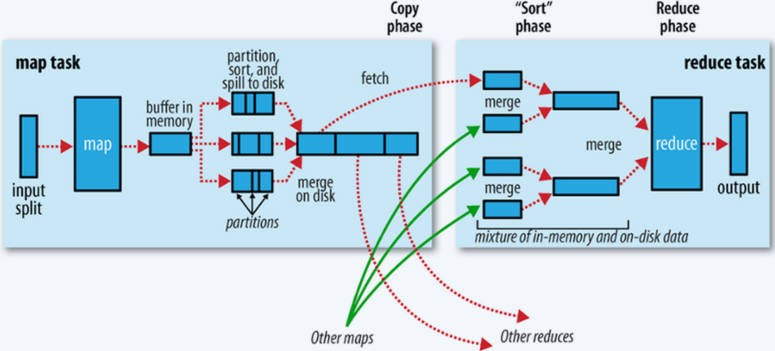
\includegraphics[width=.95\textwidth]{pics/mr_shuffle.jpg}
	\caption{Shuffle}
	\label{fig:mr-shuffle}
\end{figure}

通过以上简单的介绍, 其实已经体现了 shuffle 的作用: 1) 处理 mapper 的输出, 按照分区进行 merge; 2) 从 map 结点获取数据并 merge 作为 reduce 的输入; 3) shuffle 为猿们处理了这一繁杂的过程, 其中涉及到很多细节, 如内存中缓冲的数据如何 spill 到磁盘中, spill 文件的格式, reduce 如何拉取对应的数据等.

以上只是一个简单的介绍, 其实还有很多细节.